%% State of the art theory, concept, method relevant to address the Innovation or Entrepreneurial question/challenge. ca. 2-4 pages

\section{State of The Art}
In the discipline of IT innovation I tried to find out the existing framework to get customers' feedback while we are developing our Fog Computing solution. 
%From our research, we found out two different strategies to design and develop innovative product based on users' feedback; lean startup and design thinking. 

From my research, I found out that there are some strategies that are proved to be effective in developing innovative product based on customer feedback. I haved discussed them shortly below and based on the comparative discussion I selected and used some methods for our use case in the next section.

\subsection{Lean Startup}

One popular strategy is lean startup \citep{leanstartup} which states that efficient innovation is that one which has demand. And the biggest waste in a product development is adding the features that no customer wants. Lean methodology mainly focuses on a  Build-Measure-Learn feedback loop which is said to be at the core of the Lean Startup model\cite[p.~70]{leanstartup}. The process model is shown in Figure \ref{img:leanloop}.  

\begin{figure}[H]
  \centering
  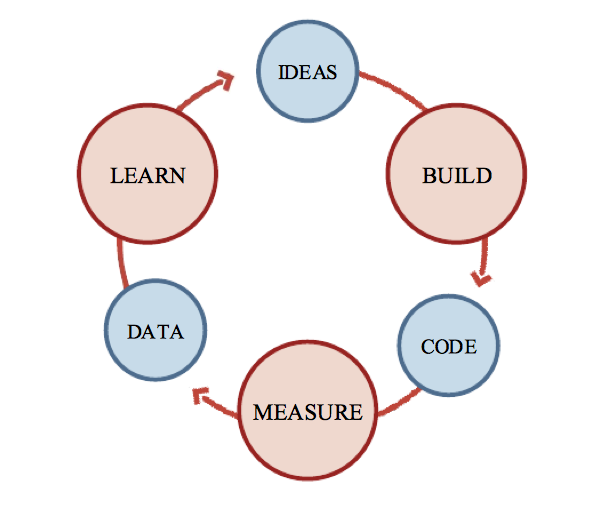
\includegraphics[width=.45\textwidth]{img/build-measure-learn.png}
  \caption{Build Measure Learn feedback loop  \cite[p.~70]{leanstartup}}\label{img:leanloop}
\end{figure}
 
The idea of lean process model is to iterate this feedback loop. That means develop the product fast, measure(test) it among the customers and learn what needs to be changed. The faster startups can iterate this process, the sooner they will learn customer feedback and be able to pivot if needed. Then the startup can start next iteration again. This way companies will be able to deliver a product fast that has customer demand, which will minimize the waste. Lean methods also says to start this iteration fast with a \ac{MVP}, and then to add features in next iterations based on customer feedback. According to Ries, most startups emphasize on individual elements of this cycle. Engineers tries to build best designed initial product, while managers focus on data and metrics. But, instead of individual priorities of team, startups should focus on minimizing the total time of this feedback loop. This way, they can learn from customer and pivot to deliver better product in next cycle.
%"individual nouns: having the best product idea or the best-designed initial product or obsessing over data and metrics. The truth is that none of these activities by itself is of paramount importance. Instead, we need to focus our energies on minimizing the total time through this feedback loop."

Also lean learning cycle can be applied to different phase of product development. From the broad level, it can be applied to overall product or even in a single feature of a product, like the color of signup button. The main idea is to learn early to avoid waste of effort, during the development of the product.

%%"Also, the lean learning cycle might be applied to different levels of a project. On a meta-level, it could be applied to the entire process, and on a micro-level, it could be applied to specific details (like the color of a signup button)." --compare paper

Lean Startup is seen to be evolved from Customer Development \cite[p.~2]{leanvsdesign}. `Customer Development Model' were introduced by Steven Gary Blank in his book `The Four Steps to the Epiphany'\citep{fstE}, where the 4 steps are customer discovery, customer validation,
customer creation and company building. According to Blank, all successful startups invent a parallel process beside product development. This process involves customer learning and discovery, and Blank stated this process as ```Customer Development', a sibling to `Product Development'."

The success of startups lies in not only great product development, but also ``Customer Development". The Customer Development model is shown in Figure \ref{img:customerdevmodel}.

\begin{figure}[H]
  \centering
  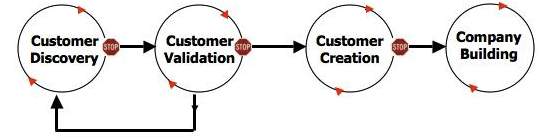
\includegraphics[width=.55\textwidth]{img/customer-development.jpg}
  \caption{Customer Development Model  \cite[p.~16]{fstE}}\label{img:customerdevmodel}
\end{figure}

This model separates out all the customer-related activities from product development. The four steps of `Customer Development' are introduced briefly below:

\textbf{Customer Discovery}: A group of identifiable users who share the same problem. The product will solve their problem.

\textbf{Customer Validation}: The market is big that a viable business can be established.

\textbf{Customer Creation}: The business can scale up by repeating sales and marketing strategies.

\textbf{Company Building}: Different Departments and operations can grow to support scale up of business.

The main idea of both these methods is same, adding a different process of ``customer development" or ``MEASURE" beside "product development" to find customers and their needs. That's how these user-centered approach help startups to adapt their product to their customer needs.

%Company departments and operational processes are created to support scale 

%"Through trial and error, hiring and firing, successful startups all invent a parallel process to product development.
%In particular, the winners invent and live by a process of customer learning and discovery. I call this process “Customer Development,” a sibling to “Product Development,” and each and every startup that succeeds recapitulates it, knowingly or not."


%"The Customer Development model of a startup starts with a simple premise: learning and discovering who a company’s initial customers will be, and what markets they are in, requires a separate and distinct process from product development."

%It was evolved from Customer Development. 


\subsection{Design Thinking}

Design Thinking is another user-centric innovation method. Similar to the lean methods, design thinking takes into account the opinion of the users and then design (develop) a solution for users. Design thinking involves extensive user research, user feedback and iteration cycles. The idea originally started in the design field where designer first listen to the customer and then come up with a design and there are some iterations to improve the design. Design thinking solves the wicked problems of users\citep{designthinkingWicked} and generate a solution based on their statements. This strategy was introduced by design consultancy firm IDEO in 2001 \citep{designthinkingIDEO}, but based on designerly methods. 


%There is another user-driven innovation strategy called ``Design Thinking". Design thinking makes use of extensive user research, feedback loops and iteration cycles. This strategy was introduced by design consultancy firm IDEO in 2001 \citep{designthinkingIDEO}, but based on designerly methods. Though it was not related to lean methods, but the basic idea was similar: identify user needs to deliver their suitable solutions. 

%Based on a user-centered approach with multi-disciplinary teams, it aims at solving complex (wicked) problems (Buchanan, 1992; Rittel, 1972) and at generating innovative solutions. 


A design thinking process model by Plattner et al. (2009) \citep{designthinkingplattner} is shown in the Figure \ref{img:designthinking}.

\begin{figure}[H]
  \centering
  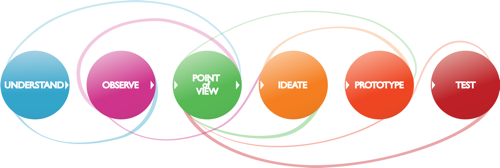
\includegraphics[width=.55\textwidth]{img/design-thinking-model.png}
  \caption{Design Thinking Process Model  \cite{designthinkingplattner}}\label{img:designthinking}
\end{figure}

The design thinking process model also consists of 6 steps as lean startup model. The key point to observe in this method is, it does not start with an idea, rather it starts directly with a user focus; probably with a problem or question. The first step `understand' is researching about the customer's problem. `Observe' means user research, where other research methods are used such as ethnographic methods and other qualitative methodology. Then `Point of View' is taken from customers, which can be direct interview. Then comes the ideation process in step `Ideate', where a solution is drafted. This solution is prototyped in next step and then `Test' is the last step where the prototype is tested with users and their feedbacks are taken. Hence, the iteration begins from 6th step `Test', but it can go to one of the previous steps based on their feedback, usually to `Point of View' step.

Though, both lean startup and design thinking has 6 steps in their process model, however, design thinking model is not entirely circular, meaning that the iteration can happen in diffrent order as opposed serial order in lean startup process model.

\begin{comment}
The model of the design thinking process (Figure 2a) describes the six steps of the process and the iteration loops that result from the last step 'test'. Notably about this process is that it does not start with an idea, but with a problem or a question, instead. Usually the ideas are developed within the process, in the fourth step 'ideation'. Before that, there is an extensive focus on the research, where 'understand' means secondary research and 'observe' means user research. Here, design thinking makes use of research methods from other disciplines such as ethnographic methods and other qualitative methodology. The acquired knowledge is then condensed into a sort of micro-theory about the problem or the user needs, the 'point of view' (POV) that is afterwards used to develop solution concepts in the 'ideation' step. It is here where innovative ideas are developed that aim at solving that previously identified problem or address the users’ needs. The selected idea is then visualized or built ('prototype') in order to test it and gather feedback from prospective users ('test'). 
According to the feedback the concept is iterated, by returning to one of the previous steps. See (Thoring & Müller, 2011b) for a more detailed description of the design thinking process.
\end{comment}

\subsection{Lean Startup Vs Design Thinking}

In one paper \citep{leanvsdesign}, I found the comparison between lean startup and design thinking processes.

The similarities of both lean startup and design thinking concepts are they foster innovation. Both are strategies to innovate a solution with minimum waste. Both concepts are user-centered approach, take user requirements to design or develop next features. Both strategies test their prototype using feedback. Lastly, both strategies encourage rapid iteration, in order to develop the desirable product for target customer segment or to pivot soon wasting minimum effort.

There are also clear differences. Firstly, scope; lean startup started with a focus on starups, whereas design thinking can be applied in general innovation. Lean startup method starts with an idea, on the other hand design thinking starts with a wicked problem. Design thinking involves extensive user research in the beginning of project and also makes use of ethnographic methods, however, in lean startup such qualitative research is not focus. In design thinking Iteration occurs after testing step and in lean startup pivoting can occur at any point, even early hypotheses can be tested with lean method.
 


%Quantitative Evaluation: Lean startup is using metric-based evaluation techniques. There are several suggestions of how hypotheses can be tested in a quantitative way (e.g. evaluating the customer acquisition costs by minimal landing pages at a small scale), and there are checklists for product-market fit and MVP definitions (Blank, 2006). Ries (2011) presents “innovation accounting” to measure the progress in validated learning. 

%Qualitative Evaluation: Design thinking uses elaborated qualitative evaluation techniques. Testing and user feedback are mainly gathered through qualitative interviews and ethnographic methods. Even though also in lean startup open interviews are used, there is not such a focus on qualitative data. Also the methods to conduct and evaluate these qualitative research methods are not as developed as in design thinking. 


Typical methods used in design decisions are Shadowing, Qualitative Interview, Paper Prototyping, Brainstorming (with specific rules), Synthesis, etc.  

Typical methods used in lean startup process are Qualitative Interview, Smoke Test, Paper Prototyping, Innovative Accounting, Split (A/B) Tests, Cohort Analysis, Funnel Metrics, Business Model Canvas, Five Whys, etc.

These methods are discussed shortly here:

\textbf{Shadowing}: Shadowing is a interview technique where candidate spends half day with another person to know about the way he thinks or works.

\textbf{Qualitative Interview}: In qualitative interview, interviewer ask open question, without giving his opinion in the questions (leading questions) and stimulate Informant to lead the conversation to get better understand of informant's opinion.

\textbf{Paper Prototyping}: Paper prototyping is a technique to test an application's user interfaces by drawing the user interface on paper and letting users interact with the paper drawing interface. This technique helps to design rapidly, simulate them fast and test the user interface quality. \citep{paperprototyping}

\textbf{Brainstorming}: is a group activity where members try to find a solution collectively by providing spontaneous ideas.

%In computer programming and software testing, smoke testing (also confidence testing, sanity testing[1][2]) is preliminary testing to reveal simple failures severe enough to (for example) reject a prospective software release. A smoke tester will select and run a subset of test cases that cover the most important functionality of a component or system, to ascertain if crucial functions of the software work correctly.
\textbf{Smoke Test}: Smoke test is early stage simple tests that can assess failures. If smoke tests fails, then we product should be developed from beginning with more care. 

\textbf{Innovative Accounting}: ``Innovation accounting is a measurement/accounting system that uses actionable metrics to evaluate how fast we are learning as a critical measure of progress toward converging on a business-valuable result", Eric Ries. \citep{leanstartup}

%A/B testing (sometimes called split testing) is comparing two versions of a web page to see which one performs better. You compare two web pages by showing the two variants (let's call them A and B) to similar visitors at the same time. The one that gives a better conversion rate, wins!
\textbf{Split (A/B) Tests}: Split A/B testing provides 2 different (solution A and B) solutions  to the users and measure which one is more preferred among users.
%Cohort analysis is a subset of behavioral analytics that takes the data from a given dataset (e.g. an eCommerce platform, web application, or online game) and rather than looking at all users as one unit, it breaks them into related groups for analysis. These related groups, or cohorts, usually share common characteristics or experiences within a defined time-span. Cohort analysis allows a company to “see patterns clearly across the life-cycle of a customer (or user), rather than slicing across all customers blindly without accounting for the natural cycle that a customer undergoes.”

\textbf{Cohort Analysis}: Cohort analysis is a subset of behavioral analytics. Cohort takes data from a given dataset and breaks them into related groups (cohorts) for analysis. Each cohort has same characteristics. This helps companies to analyse the same group of customers instead of looking at all users at once. 

\textbf{Funnel Metrics}: Funnel Metrics helps to measure the conversion rate from visitor to paid customer. \cite[p.~112]{leanstartup}

%The Business Model Canvas is a strategic management and lean startup template for developing new or documenting existing business models. It is a visual chart with elements describing a firm's or product's value proposition, infrastructure, customers, and finances.

\textbf{Business Model Canvas}: Business Movel Canvas is a visual chart to describe new or existing business model. It describes a business model listing the different elements like product's value proposition, customers, revenues etc.

\textbf{Five Whys}: Five Whys is a technique to make incremental investments and to understand the core of a problem. If ``why" is asked five times, it can help uncover the root of problem that user faces. If not asked, the core problem will be unidentified and it will come up later.\cite[p.~212]{leanstartup}

%Another user-driven innovation strategy that has become more and more popular during the last decades is “design thinking”. Based on designerly methods and principles, this strategy was developed by the design consultancy IDEO in the late 90s (Kelley & Littman, 2001). Although it is not referring to lean principles, the main idea behind it is similar: it tries to identify user needs in order to create appropriate solutions.
%Similar to lean startup, design thinking is also focusing on users or customers. Based on a user-centered approach with multi-disciplinary teams, it aims at solving complex (wicked) problems (Buchanan, 1992; Rittel, 1972) and at generating innovative solutions. Design thinking makes use of extensive user research, feedback loops and iteration cycles.

%Then there are also Design Thinking. 

%We have checked both Design Thinking and Lean Startup. 


%Different methods to perform Lean Startup or Design Thinking. 


%We selected a method. 

%Solve the problem, get the results, what customers need. 


%Perform a Ethnographic research. Who is my Customer. 


I also saw that lean startup depends more on quantitative or metric-based evaluation techniques. It measures daily page visit, new sign up number, split a/b test etc. to learn about customer preference. Design thinking depends more on qualitative evaluation. Testing and user feedback are collected by qualitative interviews and ethnographic methods. In lean startup qualitative data is not main focus.

In the next section I will consider which strategy is best suitable for us to learn customer feedback and develop the best product in minimum time.